\chapter{Plochy a ich vlastnosti}

\label{kap:plochy} % id kapitoly pre prikaz ref

V tejto kapitole popíšeme spôsoby zadania funkcií, ich výhody a nevýhody
ako aj základné definície a vety, ktoré budeme v práci používať.

\section{Funkcia daná implicitne}

\begin{definition}
    Nech $A \subseteq \mathbb{R}^n$, $B \subseteq \mathbb{R}$ sú neprázdne množiny. 
Hovoríme, že na množine $A$ je definovaná funkcia viacerých premenných
$f$, ak je daný predpis, ktorý každej n-tici $(x_1, . . . , x_n)$
z množiny $A$ priradí práve jeden prvok $f(x_1, . . . , x_n)$ z množiny $B$.
Zapisujeme 
$$f : A \to B$$
$$(x_1, . . . , x_n) \mapsto f(x_1, . . . , x_n)$$
Ak premennú $y \in B$ vyjadríme ako funkčnú hodnotu bodov $(x_1, . . . , x_n) \in A$
$$f : y = f(x_1, . . . , x_n),$$
hovoríme o explicitnom zadaní funkcie.
\end{definition}


Pri explicitne zadanej funckii je závislá premenná $y \in \mathbb{R}$ vyjadrená ako funkčná hodnota nezávislých
premenných $(x_1, . . . , x_n)\in\mathbb{R}^n$.
\\*
Funkcia zadaná implicitne je daná pomocou funkcie $$F : \mathbb{R}^n \times \mathbb{R} \to \mathbb{R}$$
$$(x_1, . . . ,x_n, y) \mapsto F(x_1, . . . , x_n, y),$$ ktorá každému prvku z $(x_1, . . . ,x_n, y) \in \mathbb{R}^{n} \times \mathbb{R}$ 
priradí určitú hodnotu \mbox{$F(x_1, . . . , x_n, y) \in \mathbb{R}$.}
Implicitne definovaná funkcia je daná nulovou hladinou tejto funkcie, teda bodmi $(x_1, . . . , x_n, y)$, 
ktoré vyhovujú rovnici $$F(x_1, . . . , x_n, y) = 0.$$  
Táto rovnica určuje vzťah medzi závislou premennou $y \in \mathbb{R}$
a nezávislými premennými $(x_1, . . . , x_n) \in \mathbb{R}^n$. 

\begin{note}
    Ak $f : \mathbb{R}^n \to \mathbb{R}$, $f: y = f(x_1, . . . , x_n)$ je funkcia a body
    $(x_1, . . . , x_n, y) \in \mathbb{R}^n \times \mathbb{R}$ vyhovujúce implicitnej rovnici 
    $$F(x_1, . . . , x_n, y) = 0$$
    sú grafom funkcie f,
    potom je funkcia f implicitne zadaná danou rovnicou.
\end{note}

Teda pre každú explicitne zadanú funkciu existuje implicitná rovnica, ktorá ju určuje.
Naopak to však neplatí. Nie každá implicitná rovnica určuje vzťah pre jedinú explicitne zadanú
funkciu. Príkladom je implicitná rovnica pre jednotkovú kružnicu $x^2 + y^2 - 1 = 0$. 


V našej práci sa zaoberáme algoritmami triangulácie implicitne definovaných funckii v $R^3$, teda odteraz
budeme pracovať iba s funkciami pre $n = 2$. Grafy takýchto funkcii budeme nazývať \textit{plochy}. 
Ďalej bude platiť, že $x$ a $y$ sú nezávislé premenné a $z$ je závislá premenná.


Aj keď sa implicitné funkcie nedajú vždy vyjadriť explicitne, pre každú spojite diferencovateľnú
implicitnú funkciu platí, že na nejakom okolí takmer každého bodu, existuje explicitná funkcia,
ktorou sa dá vyjadriť.
O tom nám hovorí nasledujúca veta.





\begin{theorem}
 (o funckií danej implicitne pre $\mathbb{R}^3$)
 
 Nech funkcia $\mathbb{R}^3 \to \mathbb{R}$ je spojite diferencovateľná. 
 Nech $(x_0, y_0, z_0) \in \mathbb{R}^3$ je bod taký, že $F(x_0, y_0, z_0) = c$.
 Ak $$\frac{\partial F}{\partial z} (x_0, y_0, z_0) \neq 0$$ potom existuje okolie 
 bodu $(x_0, y_0, z_0)$ také, že ak $(x, y)$ je dostatočne blízko $(x_0, y_0)$, 
 tak v tomto okolí existuje jediná funkcia $z = z(x ,y)$ spĺňajúca implicitnú rovnicu
 $F(x, y, z(x, y)) = c$. Navyše platí $z(x_0, y_0) = z_0$.
\end{theorem}

Pomocou explicitne zadanej funkcie nevieme vyjadriť veľa reálnych objektov, 
vieme vyjadriť len ich časti, ktoré treba následne zlepiť, 
preto je funkcia daná implicitne pri vykresľovaní povrchu veľmi obľúbená. 
Implicitne definované plochy majú oproti explicitným veľkú výhodu napríklad
v CSG modelovaní. Vďaka CSG modelovaniu vieme vytvárať pomerne komplexné
modely len používaním booleovských operácií (zjednotenie, prienik, rozdiel)
a geometrických transformácií. Tieto operácie sa aplikujú veľmi jednoducho, ak
máme plochy zadané implicitne.
!TODO! výhody a nevýhody implicitne zadaných plôch


\begin{note}
    Z vety o funkcií danej implicitne navyše vyplýva, že ak je $z = z(x,y)$ definovaná na nejakom 
    zúžení definičného oboru funkcie F podľa predchádzajúcej vety, tak $z$ je spojitá funkcia v 
    premennej x aj v premennej y. 
\end{note}

\newpage

\section{Vlastnosti funkcie danej implicitne}

Vlastnosti plôch sú dôležité pri každom algoritme modelujúcom tieto plochy. Využívame ich napríklad na detekciu ostrých hrán, 
zisťovanie zakrivenia funkcie ale aj pri rôznych dodatočných úpravách výsledkov základných algoritmov.
Ak nepoznáme vyjadrenie funkcie $z(x, y)$ môžeme jej vlastnosti získať z jej implicitnej rovnice $F(x, y, z) = 0$.


\begin{theorem}
    (derivácia funkcie danej implicitne)

    Parciálne derivácie funkcie $z(x, y)$ danej implicitne rovnicou F(x, y, z) = 0 možno vypočítať pomocou vzorca
    $$\frac{\partial z(x, y)}{\partial x} = -\frac{\frac{\partial F}{\partial x}}{\frac{\partial F}{\partial z}}$$
    a podobne 
    $$\frac{\partial z(x, y)}{\partial y} = -\frac{\frac{\partial F}{\partial y}}{\frac{\partial F}{\partial z}}$$
\end{theorem}

Normála k ploche definovanej implicitne funkciou $F(x,y,z)$ v bode $(x_0, y_0, z_0)$ je definovaná ako jednotkový 
gradient implicitnej funkcie  v tomto bode.

\begin{definition}
    Nech $f : \mathbb{R}^3 \to \mathbb{R}$ je spojite diferencovateľná funkcia. Gradient tejto 
    funkcie je definovaný ako 
    $$\nabla F(x, y, z) = (\frac{\partial F(x, y, z)}{\partial x}, \frac{\partial F(x, y, z)}{\partial y}, 
    \frac{\partial F(x, y, z)}{\partial z})$$
    a normálový vektor ako normovaný gradient
    $$N(F(x, y, z))  = \frac{\nabla F(x, y, z)}{\| \nabla F(x, y, z) \|}.$$
    \\*
    Gradient tejto funkcie v bode $(x_0, y_0, z_0)$ vypočítame dosadením $$\nabla F(x, y, z)_{\big|(x_0, y_0, z_0)}$$ 
    a normálový vektor podobne ako $$N(F(x, y, z))_{\big|(x_0, y_0, z_0)}.$$
\end{definition}

Tento výpočet gradientu, resp. normálového vektora môžeme použiť iba ak poznáme parciálne derivácie funkcie $F$ v danom bode.
V opačnom prípade musíme použiť numerické metódy na výpočet gradientu. Najčastejšie metódy používané na tento problém sú 
symetrická alebo asymetrická diferencia. O tomto probléme budeme viac písať v kapitole Numerické metódy !TODO! pridať link 

\newpage

\section{Numerické metódy}

V tejto kapitole si uvedieme numerické metódy zaoberajúce sa hľadaním riešenia rovnice $f(x) = 0$.
Presnejšie majme danú \textit{spojitú funkciu} $f: M \to \mathbb{R}, M \subset \mathbb{R}$. Hľadáme bod
$\bar{x} \in R$ taký, že $f(\bar{x}) = 0$.

Naše numerické metódy túto úlohu riešia len približne, avšak s ľubovoľnou presnosťou.

\subsection{Newton-Raphsonova metóda}

\textit{Newton-Raphsonova metóda}, známa tiež ako \textit{Newtonova metóda} je iteračná metóda používaná na riešenie
úlohy nášho typu. Snažíme sa skonštruovať postupnosť $\{x_n\}_{n=0}^\infty$ takú, že $x_n \to \bar{x}$.
Podľa Newton-Raphsonovej metódy túto požiadavku spĺňa pustupnosť bodov tvorená nasledovne: 
$$ x_{n+1} = x_n - \frac{f(x_n)}{f'(x_n)}.$$

Zastavovacích kritérií máme viacero. Prvé je ak je $f'(x_n) = 0$, druhé kritérium je počet iterácií. Tieto 
dva prípady nie sú príliš uspokojivé. Posledné zastavovacie kritérium je v prípade, ak je $f(x_n)$ dostatočne 
malé, teda sme veľmi blízko koreňa. Posledné kritérium sa dá tiež preformulovať na kritérium $|x_{n+1} - x_n|$ 
je dostatočne malé.

!TODO! obrázok

\subsection{Metóda sečníc}

\textit{Metóda sečníc} je vlastne akási modifikácia \textit{Newton-Raphsonovej metódy}. Môžeme ju použiť napríklad v prípade 
keď nepoznáme predpis $f'(x)$. V tejto metóde dotyčnicu v bode $x_n$ - $f'(x_n)$ nahradíme priamkou 
predchádzajúcou cez body $f(x_n), f(x_{n-1})$ - $\frac{f(x_n) - f(x_{n-1})}{x_n - x_{n-1}}$. Túto priamku 
nazývame \textit{sečnica}.

Iterácie v metóde sečníc teda vyzerajú nasledovne:
$$ x_{n+1} = x_n - \frac{f(x_n)}{\frac{f(x_n) - f(x_{n-1})}{x_n - x_{n-1}}}.$$

!TODO! obrázok

\subsection{Zjednodušená Newtonova metóda}

\textit{Zjednodušená Newtonova metóda} sa môžem použiť v prípade, ak \textit{Newton-Raphsonova metóda} zlyhá na prvom 
zastavovacom kritériu. Táto metóda nahrádza $f'(x_n)$ dotyčnicou v začiatočnom bode $f'(x_0)$.  

\subsection{Metóda bisekcie}

\textit{Metóda bisekcie}, známa tiež ako \textit{Metóda polenia intervalu} je založená na pozorovaní, že v okolí koreňa 
funkčné hodnoty spojitej funnkcie menia znamienko. 

Majme spojitú funkciu $f(x)$ a body $a$ a $b$, také, že $f(a) \cdot f(b) < 0$, teda funkčné hodnoty majú v týchto bodoch 
opačné znamienka. Metóda bisekcie delí tento interval na polovicu a na základe znamienka funkčnej hodonty v novom bode $s = (a+b)/2$
rozhodne, či sa koreň nachádza na intervale $(a, s)$ alebo na intervale $(s, b)$. Ak platí $f(s) = 0$, potom má funkcia v danom bode 
koreň. Daný postup sa opakuje, pokiaľ nie je splnené nejaké zo zastavovacích kritérií.

Ak sa na intervale $(a, b)$ nachádza viac koreňov, metóda bisekcie nájde aspoň jeden z nich.


numericke metody
interpolacia ?
newton ?

\newpage
\section{Triangulácia}

Usporiadanú trojicu množín $(V, E, F)$, kde $V$ je množina vrcholov daná ich súradnicami, 
$E$ je množina neorientovaných hrán daná 
dvojicou vrcholov z $V$ a $F$ je množina stien daných $n$-ticou vrcholov z $V$, kde $n \geq 3$ 
nazývame mesh.

V prípade, že všetky steny sú dané trojicou vrcholov, nazývame tento mesh trianguláciou.

Trianguláciou implicitného povrchu nazývame aproximáciu tohto povrchu trojuholníkovým meshom.

Podľa článku \textit{Adaptive implicit surface polygonization using marching triangles} \cite{akkouche2001adaptive}
vhodná triangulácia by mala spĺňať viacero podmienok. Vygenerovaný mesh by mal byť konzistentný, 
teda bez dier alebo rozpojených vrcholov //TODO pridať príklad!! , hrán alebo stien. Mal by byť topologicky homeomorfný 
so zadaným implicitným povrchom. Aproximácia by mala byť dostatočne presná a trojuholníky by mali 
byť čo najpravidelnejšie. Naviac triangulácia povrchu by sa mala prispôsobiť zakriveniu povrchu,
teda mala by vyprodukovať menšie trojuholníky v miestach s väčším zakrivením povrchu a naopak väčšie
trojuholníky v miestach s menším zakrivením.

Na tringuláciu implicitného povrchu sa používa množstvo rôznych prístupov, avšak nie každá metóda
dokáže vyprodukovať trianguláciu spĺňajúcu všetky kritéria, ktoré sme popísali. Na druhú stranu, 
presnejšie algoritmy, ktoré dokážu vyprodukovať kvalitné meshe potrebujú viac výpočtov a preto
trvajú dlhšie. 

K najrýchlejším metódam triangulácie implicitnej funkcie patria takzvané \textit{Space docomposition}
prístupy, ktoré delia priestor obsahujúci plochu na menšie bunky, napríklad kocky alebo štvorsteny.
Následne pomocou znamienka implicitnej funkcie sa vyhodnotí, či sa vrcholy buniek nachádzajú pod povrchom 
alebo nad ním. Pomocou numerických metód sa vypočítajú približné priesenčníky hrán týchto buniek s 
implicitnou funkciou a použijú sa vyhľadávacie tabuľky na zistenie triangulácie povrchu v danej bunke. 
To, že tieto metódy patria k najrýchješím nám napovedá, že nebudú príliš presné. Mnoho vedcov sa
však zameralo na tieto rýchle algoritmy a pomocou následného spracovania triangulácie sa im 
podarilo upraviť dané meshe na kvalitnejšie. Medzi najznámejšie \textit{Space docomposition} algoritmy
patrí \textit{Marching Cubes} \cite{lorensen1987marching} a \textit{Marching Tetrahedra} \cite{doi1991efficient}.

Ku kvalitnejším, avšak pomalším prístupom patria takzvané \textit{Surface tracking} prístupy.
Tieto algoritmy sa začínajú v bode ležiacom na povrchu (alebo dostatočne blízko povrchu) a 
postupne sledujú povrch a vytvárajú polygóny. Tu sa vyskytuje jedna z nevýhod implicitne zadaného
povrchu - zistiť bod ležiaci na povrchu je ťažšie ako pri explicitnom vyjadrení. Medzi najznámejšie 
\textit{Surface tracking} algoritmy patrí \textit{Marching Triangles} \cite{hilton1996marching}.



\subsection{Delaunayova triangulácia}

\begin{note}
    (difeomorfizmus)

    Pod difeomorfizmom medzi dvoma diferencovateľnými 3D manifoldmi $\mathbf{A}$ a $\mathbf{B}$ 
    môžeme rozumieť existenciu zobrazenia z $\mathbf{A}$ do $\mathbf{B}$, pričom toto zobrazenie 
    je invertibilné a spojite diferencovateľné. 
\end{note}

V tejto časti sa budeme venovať lokálnej podmienke pre potenciálny trojuholník, ktorý chceme pridať do 
výslednej triangulácie. Táto podmienka nám zaistí neprekrývajúce sa trojuholníky a teda topologickú 
ekvivalenciu implicitného povrchu a vytvorenej meshe.

Podľa článku \textit{Marching triangles: Delaunay implicit surface triangulation} \cite{hilton1997marching} 
\textit{3D Delaunayova triangulácia} ľubovoľnej množiny bodov $X\in \mathbb{R}^3$ je 
zložená zo štvorstenov takých, že pre každý z nich existuje guľa prechádzajúca cez každý z vrcholov 
štvrorstenu, ktorá neobsahuje žiadne iné body z $X$. V prípade, že body $X$ ležia na \textit{3D manifolde} 
v článku \textit{Geometric structures for three-dimensional shape representation} 
\cite{boissonnat1984geometric} odvodil \textit{J.D.Boissonnat} nasledujúcu vlastnosť. Trojuholník
lokálne difeomorfný s 3D manifoldom je v \textit{3D Delaunayovej triangulácii} ak spĺňa 
\textit{Delaunayovu vlastnosť}:

\begin{definition}
    (Delaunay face property)

    Trojuholník $\mathbf{T}$ je stenou v 3D Delaunayovej triangulácii množiny vrcholov 
    $\mathbf{X}\in \mathbb{R}^3$, ak existuje guľa prechádzajúca cez vrcholy trojuholníka 
    $\mathbf{T}$ a v tejto guli sa nenachádza žiadny ďalší vrchol z $\mathbf{X}$. 
\end{definition}

Príklad trojuholníka T_{ijk}, ktorý spĺňa Delaunayovu vlastnosť môžeme vidieť na obrázku 
\ref{obr:delaunay_face_property}. V guli predchádzajúcej cez vrcholy trojuholníka T_{ijk} 
sa nenachádza žiadny vrchol z množiny vrcholov.

Ak túto vlastnosť spĺňajú všetky trjuholníky z polyhedronu, ktorý je difeomorfný so zadaným 
\textit{3D manifoldom}, tak je tento polyhedron Delaunayovou trianguláciou zadaného povrchu pre 
množinu bodov $\mathbf{X}$.

\textit{3D Delaunayova triangulácia} je analógom k \textit{2D Delaunayovej triangulácii}, pričom
body z množiny $\mathbf{X}$ ležia na 3D povrchu namiesto 2D roviny.



Pri konštrukcii \textit{Delaunayovej triangluácie} manifoldu musí každý trojuholník spĺňať 
Delaunayovu podmienku, ktorú bola sformulovaná 



\subsection{Marching Cubes}

Algoritmus \textit{Marching Cubes} \cite{lorensen1987marching} patrí k najznámejším algoritmom používaným
na trianguláciu implicitného povrchu. Prvý krát bol prezentovaný v roku 1987. Patrí k najrýchlejším
algoritmom avšak výsledok postráda mnoho kritérií kvality triangulácie. 

---Toto chcem dať asi niekde do úvodu !TODO!


Primárna motivácia na vytvorenie algoritmu bola najmä vizuálizácia získaných dát napríklad z CT alebo MRI skenov 
využívaná v medicíne. Dnes majú vizualizácie implicitných povrchov oveľa širšie využitie.

Prístup \textit{rozdeľuj a panuj} spočíva rozdelení zložitejšieho problému na podproblémy, 
ktoré sa dajú jednoduchšie riešiť a následne tieto riešenia spojí do jedného.

Tento prístup sa rozhodli využiť aj autori algoritmu \textit{Marching Cubes}. Rozdelenie problému
spočíva v podrozdelení priestoru, v ktorom sa nachádza zadaný povrch na kocky so zvolenou dĺžkou
hrany. Následne sa pre každú kocku vypočíta, ktoré vrcholy sa nachádzajú pod povrchom (alebo na ňom) 
a ktoré nad povrchom. Keďže každá kocka má 8 vrcholov a každý vrchol môže nadobudnúť hodnotu $1$, ak sa 
nachádza pod povrchom alebo na ňom, alebo hodnotu $0$, ak sa nechádza nad povrchom, exisuje práve 
$2^8 = 256$ možností. Vďaka symetriám sa však autorom podarilo znížiť tento počet len na 14 rôznych možností.
Pre tieto možnosti vytvorili tabuľku, kde pomocou 8 bitového binárneho čísla označujúceho charakteristiku
kocky vyhľadávali dané triangulácie.

Približná poloha priesečníka s hranou kocky sa dá vypočítať napríklad pomocou lineárnej inerpolácie, avšak 
dajú sa použiť aj presnejšie, avšak pomalšie, interpolácie vyšších rádov.

Výstupom algotitmu sú okrem triangulácie aj normály vo vrcholoch triangulačných trojuholníkov vypočítané pomocou lineárnej
interpolácie normalizovaného gradientu získaného pomocou \textit{centrálnej diferencie} vo vrcholoch prerozdelených kociek. 
Tieto normály sa používajú najmä na čo najpresnejšie tieňovanie triangulácie.


\subsection{Marching Triangles}

Algortimus \textit{Marching Triangles} \cite{hilton1996marching} patrí do skupiny algoritmov založených na takzvanom 
sledovaní povrchu. Prvý krát bol prezentovaný v roku 1996. Oproti algoritmu \textit{Marching Cubes} je pomalší, avšak
produkuje kvalitnejšiu trianguláciu. 

Algoritmus začína v počiatočnom bode na povrchu plochy. Následne vytvorí prvý trojuholník na povrchu a hrany vzniknutého 
trojuholníka vloží do zoznamu hraničných hrán. 
Opakujúc sériu krokov postupne zväčšuje trianguláciu. V každom z týchto krokov zo zoznamu vyberie jednu hranu $E$. 
Táto hrana susedí práve s jedným trojuholníkom. V rovine susedného trojuholníka vytvorí kolmicu na hranu $E$
(podľa \ref{obr:new_vertex}) a následne na nej bod $V$ v nejakej vzdialenosti $k$. 

\begin{figure}
    \centerline{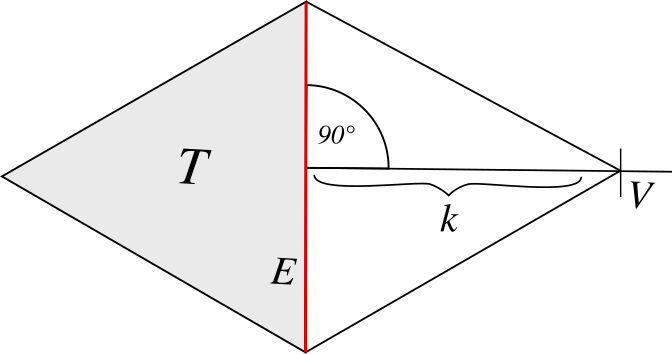
\includegraphics[width=0.6\textwidth]{images/new_vertex}}
    \caption[Vytváranie nového vrcholu $V$ v rovine susedného trojuholníka]{Vytváranie nového vrcholu v rovine susedného trojuholníka}
    %id obrazku, pomocou ktoreho sa budeme na obrazok odvolavat
    \label{obr:new_vertex}
\end{figure}

Vzdialenosť $k$ môže byť daná fixne alebo môže mať premenlivú veľkosť, v pôvodnom algoritme je táto vzdialenosť fixná. 
Následne sa tento bod pomocou numerických metód sprojektuje na povrch a overí sa \textit{Delaunayova podmienka} pre novovzniknutý 
trojuholník. 
Ak trojuholník spĺňa \textit{Delaunayovu podmienku}, pridá sa do triangulácie. V opačnom prípade sa snažíme vytvoriť iný trojuholník 
skladajúci sa z pôvodnej hrany a vrcholov, ktoré sú susedné k vrcholom tejto hrany. V prípade, že aj tieto trojuholníky nespĺňajú 
\textit{Delaunayovu podmienku}, pokúsime sa vytvoriť trojuholník s hraničným vrcholom už existujúcej triangulácie ktorý pretína
guľu kontrolujúcu $Delaunayovu podmienku$, ak taký existuje. Ak ju však ani tento trojuholník nesplní, testovanie danej hrany sa skončí.

Ak sa v danom kroku algoritmu pridá nejaký trojuholník do triangulácie, tak odoberieme hranu, s ktorou sme pracovali zo zoznamu a 
vložíme do nej novovytvorené hrany nachádzajúce sa na hranici.

Tento postup sa opakuje pokiaľ existujú neskontrolované hrany na hranici triangulácie.

\newpage

\section{Singulárne body a krivky}

Singulárne body implicitne danej funkcie sú také body, kde $\nabla F(x, y, z) = 0$. Tieto body nemusia byť nutne izlované, 
v tom prípade hovoríme o singulárnych krivkách. 

Singulárne body a krivky sa vyskytujú napríklad pri CSG modelovaní.

\medskip

!TODO! obrázok singulárnej krivky a bodu, ukážka funkcie v ktorej sa vyskytuje singulárna 
krivka a popísanie metód hľadania týchto bodov a kriviek

\medskip

zakrivenie funkcie



delaunayova podmienka
algoritmy triangulacie






